\documentclass[12pt]{article}
\usepackage[letterpaper,margin=0.7in,headheight=15pt,headsep=16pt,footskip=25pt]{geometry}
\usepackage{tikz,array,fancyhdr,lmodern}
\renewcommand{\familydefault}{\sfdefault}
\pagestyle{fancy}\fancyhf{}\renewcommand{\headrulewidth}{0.35pt}
\fancyhead[L]{\small Week 29 / Two-length builders encore / Grades K--5}
\fancyfoot[L]{\scriptsize Bellingham Math Circle / Week 29 / W29-BON-v1}\fancyfoot[R]{\scriptsize\thepage}
\setlength{\parindent}{0pt}\setlength{\parskip}{9pt}
\newcommand{\problem}[2]{\par\textbf{Problem #1:} #2\par}
\newcommand{\lines}[1]{\foreach \y in {1,...,#1}{\par\vspace{20pt}\hrule height 0.3pt\relax}}
\newcommand{\rod}[2]{\draw[fill=gray!12] (#1,0) rectangle ++(#2,0.65);\foreach \i in {1,...,#2}\draw[gray] (#1+\i,0)--(#1+\i,0.65);\node at (#1+#2/2,0.325){#2};}
\newcommand{\wordrows}{\begin{tabular}{|p{1.7in}|}\hline\rule{0pt}{40pt}\\\hline\rule{0pt}{40pt}\\\hline\rule{0pt}{40pt}\\\hline\rule{0pt}{40pt}\\\hline\rule{0pt}{40pt}\\\hline\rule{0pt}{40pt}\\\hline\end{tabular}}
\begin{document}
Build beside the page with whole rods of length 3 and 4. A word gives their lengths from the fixed left end to the right. Different orders count as different words. Rods of the same length are alike.
\begin{center}
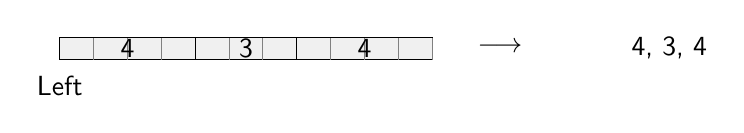
\begin{tikzpicture}[x=0.43cm,y=0.43cm]\rod{0}{4}\rod{4}{3}\rod{7}{4}\node[below] at (0,-0.2){Left};\node at (13,0.35){$\longrightarrow$};\node at (18,0.35){4, 3, 4};\end{tikzpicture}
\end{center}
\problem{1}{Build lengths 7, 10, and 14 beside the page. Find every word for each length.}
\vspace{8pt}
\begin{minipage}[t]{.31\linewidth}\centering 7\par\wordrows\end{minipage}\hfill\begin{minipage}[t]{.31\linewidth}\centering 10\par\wordrows\end{minipage}\hfill\begin{minipage}[t]{.31\linewidth}\centering 14\par\wordrows\end{minipage}
\vspace{16pt}
\lines{6}
\newpage
\problem{2}{Find every 3-and-4 word that builds 18. Find a rule that uses word counts for shorter lengths to count the words for any new length.}
\vspace{10pt}
\begin{tabular}{|p{2.65in}|p{2.65in}|}\hline\rule{0pt}{44pt}&\\\hline\rule{0pt}{44pt}&\\\hline\rule{0pt}{44pt}&\\\hline\rule{0pt}{44pt}&\\\hline\rule{0pt}{44pt}&\\\hline\rule{0pt}{44pt}&\\\hline\end{tabular}
\vspace{12pt}
\lines{7}
\newpage
Use only the sealed box: four 3-rods and three 4-rods. Keep the rods you use and the rods left over in two separate lanes. Do not borrow more rods.
\begin{center}
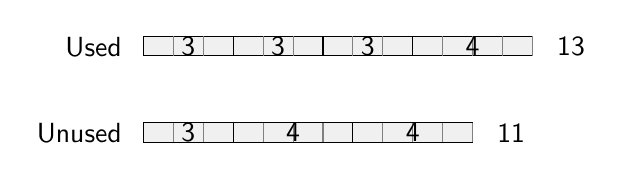
\begin{tikzpicture}[x=0.38cm,y=0.38cm]
\node[left] at (-.4,.3){Used};\rod{0}{3}\rod{3}{3}\rod{6}{3}\rod{9}{4}\node[right] at (13.5,.3){13};
\begin{scope}[yshift=-1.1cm]\node[left] at (-.4,.3){Unused};\rod{0}{3}\rod{3}{4}\rod{7}{4}\node[right] at (11.5,.3){11};\end{scope}
\end{tikzpicture}
\end{center}
\problem{3}{With this box, make lengths 6, 9, 10, 19, and 22, or show why a length cannot be made. For each successful build, what length do the unused rods make?}
\vspace{6pt}
\begin{tabular}{|p{.55in}|p{2.1in}|p{2.1in}|}\hline Target&Used rods&Unused rods and length\\\hline\rule{0pt}{41pt}6&&\\\hline\rule{0pt}{41pt}9&&\\\hline\rule{0pt}{41pt}10&&\\\hline\rule{0pt}{41pt}19&&\\\hline\rule{0pt}{41pt}22&&\\\hline\end{tabular}
\vspace{12pt}
\problem{4}{The whole box has length 24. What rule links the targets that can be made and the lengths left over? Divide all seven rods into two rows of equal length.}
\lines{5}
\newpage
For the next problems, you may use as many copies of each stated rod length as you need. Set the sealed box aside.
\problem{5}{Test three separate sets of rod lengths: 3, 5, 8; 3, 5, 7; and 3, 5, 4. For each set, find all targets it can make that 3 and 5 cannot, or explain why there are no new targets.}
\vspace{8pt}
\begin{tabular}{|p{.8in}|p{1.9in}|p{2.6in}|}\hline Added rod&New targets&Reason\\\hline\rule{0pt}{66pt}8&&\\\hline\rule{0pt}{66pt}7&&\\\hline\rule{0pt}{66pt}4&&\\\hline\end{tabular}
\vspace{12pt}
\problem{6}{Build 16 and 24 with the fewest rods. For each target, try once with lengths 3 and 5, and once with lengths 3, 5, and 8. Can a new rod change the fewest-rod answer without adding any reachable targets?}
\vspace{6pt}
\begin{tabular}{|p{.75in}|p{2.3in}|p{2.3in}|}\hline Target&3 and 5&3, 5, and 8\\\hline\rule{0pt}{49pt}16&&\\\hline\rule{0pt}{49pt}24&&\\\hline\end{tabular}
\lines{3}
\end{document}
